\section{DBSCAN}

\begin{frame}{From k-Means to Density-Based Clustering}
\begin{itemize}
  \item In k-means, every example must be assigned to one of $k$ clusters.
  \pause
  \item That works well for compact Euclidean groups, but it can fail on non-convex structure and outliers.
  \pause
  \item DBSCAN changes the viewpoint from centroids to local density.
  \pause
  \item Now the goal is to recover dense regions and leave sparse points as noise.
\end{itemize}
\end{frame}

\begin{frame}{Why DBSCAN?}
\begin{columns}[T]
\column{0.52\textwidth}
\begin{itemize}
  \item Input: examples $x_1,\dots,x_n \in \mathbb{R}^d$ with no target labels.
  \pause
  \item Output: clusters plus points labeled as noise.
  \pause
  \item Unlike k-means, the method does not require specifying the number of clusters in advance.
\end{itemize}

\pause
\column{0.48\textwidth}
\textbf{Typical uses}
\begin{itemize}
  \item spatial clustering,
  \pause
  \item grouping embeddings with irregular shape,
  \pause
  \item exploratory outlier screening,
  \pause
  \item structure discovery when some points should remain unassigned.
\end{itemize}
\end{columns}

\pause
\begin{rlintuition}
k-means looks for centroids. DBSCAN looks for dense regions.
\end{rlintuition}
\end{frame}

\begin{frame}{Formal Setup}
\begin{columns}[T]
\column{0.52\textwidth}
\begin{itemize}
  \item Let $X=\{x_1,\dots,x_n\}$ with each $x_i \in \mathbb{R}^d$.
  \pause
  \item DBSCAN uses two parameters:
  \[
    \varepsilon > 0,
    \qquad
    \text{MinPts} \in \mathbb{N}.
  \]
  \pause
  \item Here $\varepsilon$ is a neighborhood radius and $\text{MinPts}$ is a minimum local count.
  \pause
  \item The method classifies points according to how many nearby examples they have.
\end{itemize}

\pause
\column{0.48\textwidth}
\centering
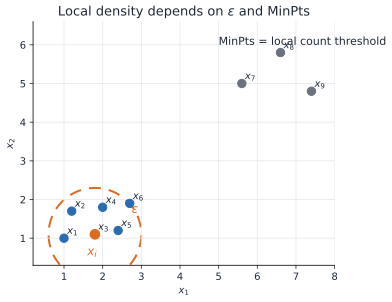
\includegraphics[width=\textwidth]{figures/dbscan/dbscan_formal_setup.pdf}
\end{columns}
\end{frame}

\begin{frame}{The $\varepsilon$-Neighborhood}
\begin{columns}[T]
\column{0.53\textwidth}
\begin{itemize}
  \item For one example $x_i$, define its $\varepsilon$-neighborhood by
  \begin{equation}
    N_\varepsilon(x_i)
    =
    \{x_j \in X : \|x_j-x_i\|_2 \le \varepsilon\}.
    \label{eq:eps-neighborhood}
  \end{equation}
  \pause
  \item This is the set of all examples within radius $\varepsilon$ of $x_i$.
  \pause
  \item The neighborhood size $|N_\varepsilon(x_i)|$ is the local density signal used by DBSCAN.
\end{itemize}

\pause
\column{0.47\textwidth}
\centering
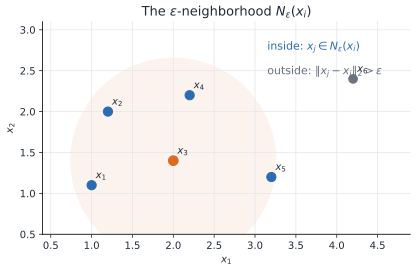
\includegraphics[width=\textwidth]{figures/dbscan/dbscan_eps_neighborhood.pdf}
\end{columns}
\end{frame}

\begin{frame}{Core, Border, and Noise Points}
\begin{columns}[T]
\column{0.53\textwidth}
\begin{itemize}
  \item A point $x_i$ is a \textbf{core point} if
  \begin{equation}
    |N_\varepsilon(x_i)| \ge \text{MinPts}.
    \label{eq:core-point}
  \end{equation}
  \pause
  \item A point $x_i$ is a \textbf{border point} if it is not a core point, but it lies in the $\varepsilon$-neighborhood of some core point.
  \pause
  \item A point $x_i$ is \textbf{noise} if it is neither core nor border.
\end{itemize}

\pause
\column{0.47\textwidth}
\centering
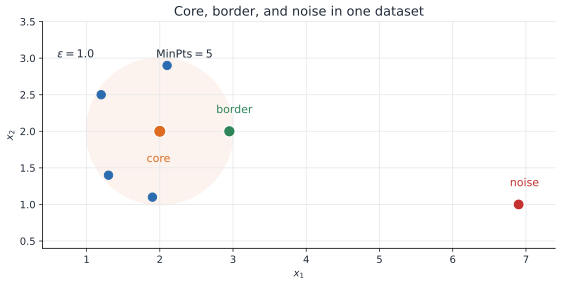
\includegraphics[width=\textwidth]{figures/dbscan/dbscan_point_types.pdf}
\end{columns}
\end{frame}

\begin{frame}{Direct Density Reachability}
\begin{columns}[T]
\column{0.53\textwidth}
\begin{itemize}
  \item A point $x_j$ is directly density-reachable from $x_i$ if
  \begin{itemize}
    \item $x_j \in N_\varepsilon(x_i)$, and
    \item $x_i$ is a core point.
  \end{itemize}
  \pause
  \item The relation is directional because the starting point must be core.
  \pause
  \item Border points can be directly density-reachable from core points, but they do not expand a cluster further.
\end{itemize}

\pause
\column{0.47\textwidth}
\centering
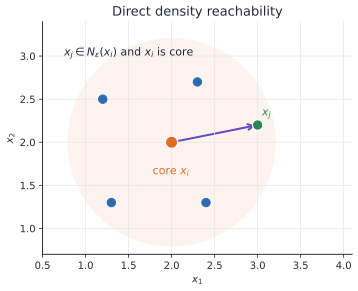
\includegraphics[width=\textwidth]{figures/dbscan/dbscan_direct_reachability.pdf}
\end{columns}
\end{frame}

\begin{frame}{Density Reachability and Connectivity}
\begin{columns}[T]
\column{0.54\textwidth}
\begin{itemize}
  \item A point $x_j$ is density-reachable from $x_i$ if there exists a chain
  \[
    x_i = x^{(1)}, x^{(2)}, \dots, x^{(m)} = x_j
  \]
  such that each $x^{(t+1)}$ is directly density-reachable from $x^{(t)}$.
  \pause
  \item Two points are density-connected if they are both density-reachable from some common core point.
  \pause
  \item DBSCAN clusters are exactly the maximal density-connected sets.
\end{itemize}

\pause
\column{0.46\textwidth}
\centering
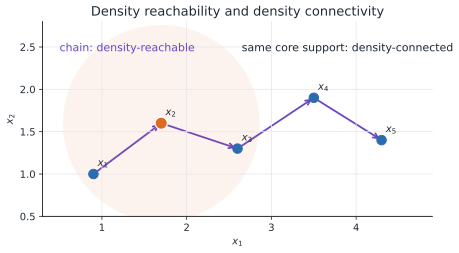
\includegraphics[width=\textwidth]{figures/dbscan/dbscan_density_connectivity.pdf}
\end{columns}
\end{frame}

\begin{frame}{How a DBSCAN Cluster Grows}
\centering
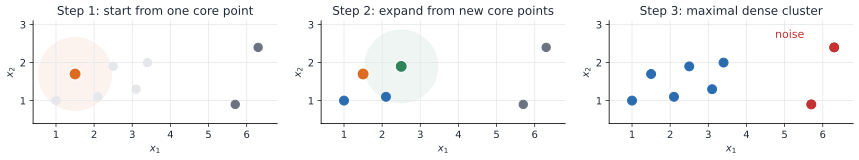
\includegraphics[width=0.97\textwidth]{figures/dbscan/dbscan_cluster_growth.pdf}

\vspace{0.35em}
\begin{itemize}
  \item Start from one unvisited core point.
  \pause
  \item Add all points in its $\varepsilon$-neighborhood.
  \pause
  \item If one of those added points is also core, expand again from that point.
  \pause
  \item Continue until no more density-reachable points remain.
  \pause
  \item Then start again from another unvisited core point.
\end{itemize}
\end{frame}

\begin{frame}{Basic DBSCAN Algorithm}
\begin{enumerate}
  \item For each unvisited example, compute its $\varepsilon$-neighborhood.
  \pause
  \item If the point is not core, mark it temporarily as noise or border.
  \pause
  \item If the point is core, start a new cluster.
  \pause
  \item Repeatedly add all density-reachable points to that cluster.
  \pause
  \item Continue until all examples are processed.
\end{enumerate}
\end{frame}

\begin{frame}{Worked Numerical Example}
\small
\begin{itemize}
  \item Let
  \[
    x_1=(0,0),\quad x_2=(0,1),\quad x_3=(1,0),\quad x_4=(5,5),\quad x_5=(5,6),
  \]
  and choose $\varepsilon = 1.5$ and $\text{MinPts}=3$.
  \pause
  \item Then
  \[
    N_\varepsilon(x_1)=\{x_1,x_2,x_3\},
  \]
  so $|N_\varepsilon(x_1)|=3$ and $x_1$ is a core point.
  \pause
  \item Similarly, $x_2$ and $x_3$ are also core points.
  \pause
  \item But
  \[
    N_\varepsilon(x_4)=\{x_4,x_5\},
  \]
  so $x_4$ is not core, and neither is $x_5$.
\end{itemize}
\end{frame}

\begin{frame}{Worked Numerical Example: Result}
\small
\begin{itemize}
  \item Since $x_1$, $x_2$, and $x_3$ are density-connected, they form one cluster.
  \pause
  \item Points $x_4$ and $x_5$ do not meet the core condition and are not attached to any core point.
  \pause
  \item Therefore the output is:
  \[
    C_1 = \{x_1,x_2,x_3\},
    \qquad
    \text{noise} = \{x_4,x_5\}.
  \]
  \pause
  \item This is the key qualitative difference from k-means: some points remain unassigned.
\end{itemize}
\end{frame}

\begin{frame}{What the Parameters Control}
\begin{columns}[T]
\column{0.5\textwidth}
\textbf{If $\varepsilon$ is too small}
\begin{itemize}
  \item neighborhoods are tiny,
  \pause
  \item many points fail the core test,
  \pause
  \item the method may label too many points as noise.
\end{itemize}

\pause
\column{0.5\textwidth}
\textbf{If $\varepsilon$ is too large}
\begin{itemize}
  \item neighborhoods overlap too much,
  \pause
  \item separate groups may merge,
  \pause
  \item outliers may be absorbed into clusters.
\end{itemize}
\end{columns}

\pause
\vspace{0.35em}
\footnotesize Increasing $\text{MinPts}$ makes the core condition stricter and usually produces fewer core points.
\end{frame}

\begin{frame}{Why Scaling Still Matters}
\begin{itemize}
  \item DBSCAN also depends on a distance computation, so feature scaling still matters.
  \pause
  \item If one feature dominates Euclidean distance, the $\varepsilon$-neighborhoods can become misleading.
  \pause
  \item Therefore the same preprocessing lesson from k-NN and k-means still applies here.
\end{itemize}
\end{frame}

\begin{frame}{DBSCAN Versus k-Means}
\begin{columns}[T]
\column{0.5\textwidth}
\textbf{k-means}
\begin{itemize}
  \item requires $k$ in advance,
  \pause
  \item assigns every point,
  \pause
  \item favors compact Euclidean groups,
  \pause
  \item is sensitive to outliers.
\end{itemize}

\pause
\column{0.5\textwidth}
\textbf{DBSCAN}
\begin{itemize}
  \item uses $\varepsilon$ and $\text{MinPts}$,
  \pause
  \item can label noise,
  \pause
  \item can recover non-convex dense regions,
  \pause
  \item struggles when cluster densities vary strongly.
\end{itemize}
\end{columns}
\end{frame}

\begin{frame}{When DBSCAN Works and When It Fails}
\begin{columns}[T]
\column{0.5\textwidth}
\textbf{DBSCAN often works well when}
\begin{itemize}
  \item clusters are separated by low-density regions,
  \pause
  \item some points should be treated as noise,
  \pause
  \item cluster shapes are irregular,
  \pause
  \item one distance scale is meaningful.
\end{itemize}

\pause
\column{0.5\textwidth}
\textbf{DBSCAN can fail when}
\begin{itemize}
  \item cluster densities differ strongly,
  \pause
  \item the correct $\varepsilon$ is unclear,
  \pause
  \item high-dimensional distances become weak,
  \pause
  \item the representation has poor geometry.
\end{itemize}
\end{columns}
\end{frame}

\begin{frame}{DBSCAN and Outlier Detection}
\begin{itemize}
  \item DBSCAN is a clustering method, but it also marks some points as noise.
  \pause
  \item Therefore it provides a simple density-based entry point to outlier detection.
  \pause
  \item However, its noise label is only as good as the chosen distance, $\varepsilon$, and $\text{MinPts}$.
  \pause
  \item So DBSCAN is useful for exploratory outlier screening, not a universal anomaly detector.
\end{itemize}
\end{frame}

\begin{frame}{Summary}
\begin{itemize}
  \item DBSCAN defines local neighborhoods using a radius $\varepsilon$.
  \item Core points satisfy the minimum-density condition $|N_\varepsilon(x_i)| \ge \text{MinPts}$.
  \item Clusters are formed by density reachability and density connectivity.
  \item Unlike k-means, DBSCAN can recover non-convex groups and leave noise unassigned.
  \item The result depends strongly on the distance, scaling, $\varepsilon$, and $\text{MinPts}$.
\end{itemize}
\end{frame}

\begin{frame}{Lab Connection}
\begin{itemize}
  \item Implement the computational core of DBSCAN with NumPy: neighborhood queries, core-point test, and cluster expansion.
  \item Compare DBSCAN with k-means on one dataset containing non-convex structure or visible noise.
  \item Report how changing $\varepsilon$ and $\text{MinPts}$ alters the number of clusters and the number of noise points.
  \item Explain one example where DBSCAN succeeds and one where it fails.
\end{itemize}
\end{frame}
